\section{Architectures Of Deep Neural Networks}

\begin{wrapfigure}[26]{r}{0.42\textwidth}
	\begin{center}
		\scalebox{0.45}{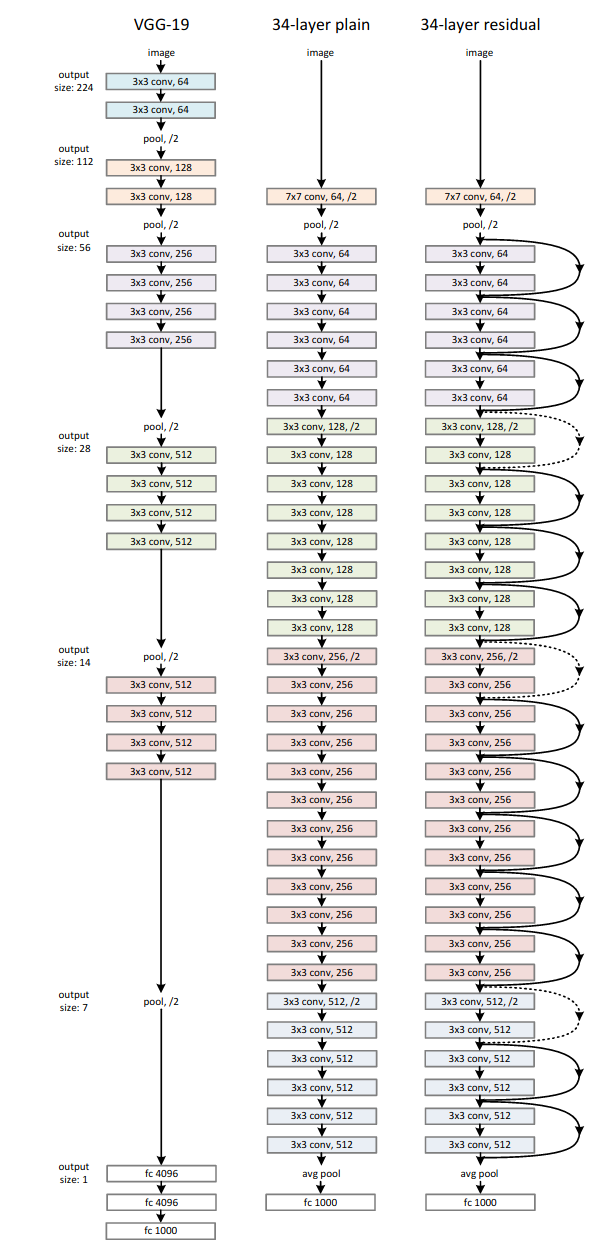
\includegraphics{resnet_comp.png}}
	\end{center}
		\caption{Examples of 16-layer VGG, Plain 34-layer, and 34-layer ResNet Network 
		Architectures}
\end{wrapfigure}

When it comes to building a neural network, one has to establish its
architecture. In this context an architecture is a blueprint of how layers are arranged and interconnected.
It is particularly important, when the network increases in complexity. Object
classification + localization being a demanding task for a network to solve,
we have adopted a published and well-tested architecture for the task --
ResNet. The particular architecture we have tried to imitate titled 
\textit{DECOLLE}, was first developed by \citeA{kaiser2018synaptic} and later
enhanced by \citeA{barchid2021deep}. \textit{DECOLLE} Neural Network adopts 
properties of classical ResNet model architecture as well as a pyramidal structure that
was proposed by \citeA{pyramid}. 


\subsection{ResNets}


To begin with the cornerstone of our architecture, ResNet is named from its property of convolutional layers which residually connect to one another(\citeA{resnet}).
According to \citeA{resnet}
addition of residual connections improves models' convergence, or ability for the
models' loss to move towards a minimum in a decreasing trend. While
ResNets converge faster than their plain counterparts, their complexity is much lower than the complexity of other well performing Visual Geometry
Group (VGG) Networks given the same depth (3.6 billion FLOPs (Float Point 
Operations) vs. 19.6 billion FLOPs) (\citeA{resnet}). 

\subsection{Comparing Model Performance}
To compare networks' performance, one has to understand how it is measured and what
constitutes is as an accurate model. Comparing accuracy of predicting the right class is not itself sufficient for the task of object detection/localization. Thus,
two additional performance metrics have been adapted: Mean Average Precision (mAP) and
Intersection of Union (IoU). Firstly, mAP for the purposes of Object
Detection is well-defined in the paper by \citeA{evaluation}. According to the authors,
mAP is the mean of Average Precision of the model for all the classes in the dataset. It is
calculated using the following equation.


\begin{equation}
	\textbf{mAP} = \frac{1}{N} * \sum_{i = 1}^{N} \textbf{AP}_i
\end{equation}

\begingroup
\fontsize{7pt}{9pt}\selectfont
\begin{enumerate}
	\item[]  \begin{center} AP = Average Precision, \end{center}
	\item[] \begin{center}  N = number of classes. \end{center}
\end{enumerate}
\endgroup


Next, IoU is the area of overlap of ground-truth boxes and the model's detected box output;
the higher the IoU the better performance of the model. Intersection of Union can be 
represented as follows.

\begin{equation}
	\textbf{IoU} = |A \cap B| \div  |A \cup B| = |I| \div |U|
\end{equation}

\begingroup
\fontsize{7pt}{9pt}\selectfont
\begin{enumerate}
	\item[]  \begin{center} I = Intersection area, \end{center}
	\item[] \begin{center}  U = Union area. \end{center}
\end{enumerate}
\endgroup


\subsection{Pyramidal Architecture of Neural Network}


Pyramidal structure of a Neural Network refers to the shape of the layers as the model
gets deeper. With each layer, dimensions of convolutional layers double.
For example, the first convolutional layer would have an input dimension equal to number of
channels in the image (3 channels for RGB images vs. 1 for greyscale). The same layer would have an output
dimension of 32, with next layer input equal to previous layer's output. The second layer
would have the dimension of 64 (half of the previous layer's output) and so on (\citeA{pyramid}).

For the purposes of our network, pyramidal structure of a neural network is leveraged using
Encoder-Decoder model. When an image is passed through the shrinking layers of the Encoder
Pyramid, it looses resolution as well as contextual information; however when the image
leaves the encoder and is located in the hidden state, it is fully comprised of
the semantic information about the image (what object is on the picture and where it is
located). Furthermore, in order to localize an object on an image the model has never 
encountered before, it must be able to place the semantic information in context. 
This is where Decoder comes into play, being the reverse of an Encoder, the convolutional
layers of decoder reduce in size until desired dimensions. The decoder is residually
connected to encoder, and thus it gains contextual information about the image through
every pass of decoder's layer.

In the end, in order to extract meaningful information, the last decoder layer is connected to Fully Connected linear layers that output predicted class, as well as
detected box coordinates.
 

\section{Implementation}

\subsection{Architecture of the Model Used}

\begin{figure}[h]
	\begin{center}
		\scalebox{0.4}{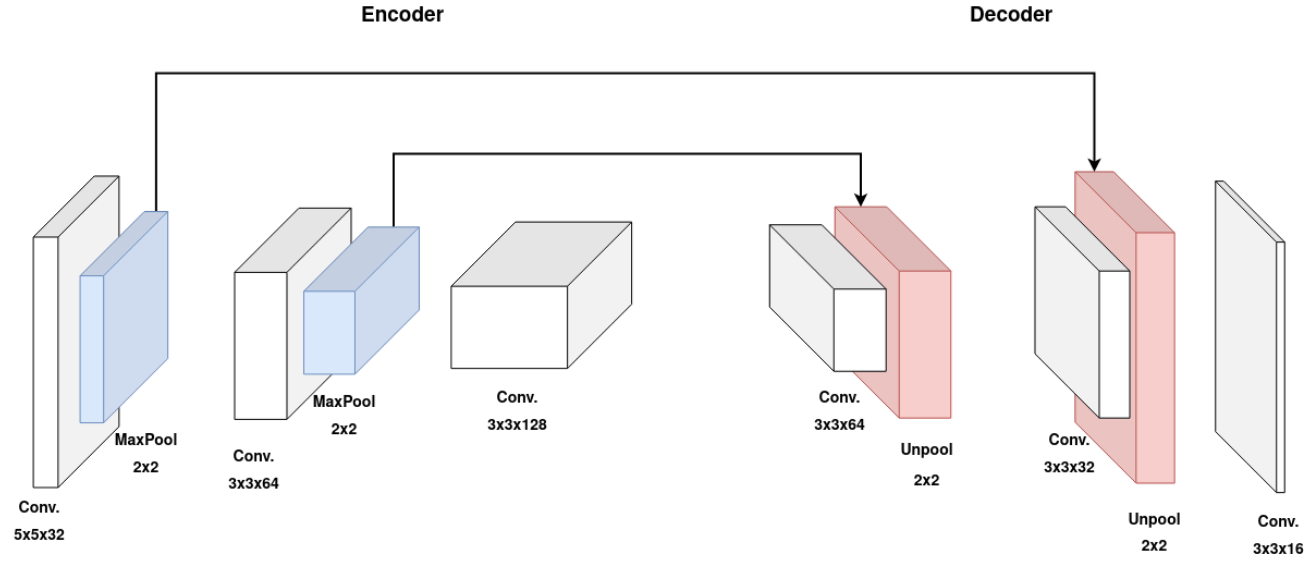
\includegraphics{barchid_SED.png}}
	
	\end{center}
	\caption{Sketch of the model's architecture. White layers represent convolutional layers,
	blue represent pooling layers, and red unpooling layers}
\end{figure}

Architecture developed by \citeA{barchid2021deep} was the target to replicate. The model is based
on Encoder-Decoder architecture with residually connecting layers akin to ResNets.

\subsection{PyTorch}

The main package that allowed us to develop such a complex model was PyTorch. PyTorch
is an open-source machine learning/deep learning library and framework for Python, 
which allows users to develop and ship high performance models (\citeA{pytorch}). This library
eliminates the need of `from scratch`' development of the most important methods in machine learning,
such as activation functions, and model architecture assembly.


\subsection{Spiking Neurons}

Given the complexity of SNNs and the integration of LIF
into the network, we used a package that allows the use LIF within a PyTorch model -- 
\href{https://snntorch.readthedocs.io/en/latest/snntorch.html}{\textit{snnTorch}}. 
snnTorch also allowed us to integrate backpropogation for spiking neural networks
with one line.

\begin{lstlisting}[language=Python, caption=Leaky-Integrate-and-Fire using snnTorch]
	import snntorch as snn
	spike_grad = surrogate.fast_sigmoid(slope=25)
	beta = 0.5

	lif1 = snn.Leaky(beta=beta, spike_grad=spike_grad)

\end{lstlisting}

\subsection{The End Product}


As we conclude, we should note we were challenged beyond our capabilities within the allotted time; this was known going into the project and as such we worked keeping these constraints in mind. For instance, SNNs when implemented on conventional GPUs are extremely memory hungry due to the need to store membrane potential information. This feature of SNNs caused a constraint in terms of hardware capabilities that were unavailable to us. In another instance, we faced challenges implementing a model based on literature. While \citeA{barchid2021deep} provided great detail on their results, they lack the necessary information to implement their model. Lastly, we faced challenges when integrating snnTorch with PyTorch in a scale this big. Indeed, following the documentation of snnTorch, it is difficult to interpret the methodologies required to develop a model beyond a simple sequential architecture. 


Though challenged, we should also note the accomplishments of the project; we have developed a custom dataloader for the MSCOCO dataset, reconstructed the general model of \citeA{barchid2021deep} network, and explored \textit{snnTorch} and \textit{PyTorch} on a smaller dataset (MNIST). All of which contributes to our ultimate goal of understanding the applications of neuroscience on a much deeper level. 

All our attempts at implementation of the network are attached with this report and can also be found on the \href{https://github.com/arsalikhov/PSYCH420_final_project}{GitHub page} for this project.

